% Copyright 2004 by Till Tantau <tantau@users.sourceforge.net>.
%
% In principle, this file can be redistributed and/or modified under
% the terms of the GNU Public License, version 2.
%
% However, this file is supposed to be a template to be modified
% for your own needs. For this reason, if you use this file as a
% template and not specifically distribute it as part of a another
% package/program, I grant the extra permission to freely copy and
% modify this file as you see fit and even to delete this copyright
% notice. 

\documentclass{beamer}
\setbeamertemplate{navigation symbols}{}
%\useoutertheme{shadow}
\setbeamertemplate{headline}{}

\usepackage{amssymb}
\usepackage{amsthm}
\usepackage{amstext}
\usepackage{amsbsy}
\usepackage{amscd}
\usepackage{enumerate}
\usepackage{chngpage}
\usepackage{mathtools}
\usepackage{amsmath}
\usepackage{hyperref}
\usepackage{tikz}
%\usepackage{stmaryrd}
\usepackage{color}
\usepackage{wrapfig}

\theoremstyle{plain}


\newtheorem{alg}{Algorithm}
\newtheorem{thm}{Theorem}[section]
\newtheorem{lem}[thm]{Lemma} 
\newtheorem{cor}[thm]{Corollary}
\newtheorem{prop}[thm]{Proposition}
\theoremstyle{definition}
\newtheorem{defn}[thm]{Definition}
\newtheorem{question}[thm]{Question}
\newtheorem{conj}[thm]{Conjecture}
\newtheorem{obs}[thm]{Observation}
\newtheorem{claim}[thm]{Claim}
\newtheorem{rmk}[thm]{Remark}

\newcommand{\Z}{\mathbb Z}
\newcommand{\N}{\mathbb N}
\newcommand{\R}{\mathbb R}
\newcommand{\C}{\mathbb C}
\newcommand{\Q}{\mathbb Q}
\newcommand{\F}{\mathbb F}
\newcommand{\Fp}{\mathbb{F}_p}
\newcommand{\Fq}{\mathbb{F}_q}

\newcommand{\sthat}{\,|\,}
\newcommand{\stp}[1]{\st\left(#1\right)}

\newcommand{\hal}[1]{\mathrm{hal}(#1)}
\newcommand{\gal}[1]{\mathrm{gal}(#1)}

\newcommand{\reals}{\mathbb{R}}
\newcommand{\hreals}{\prescript{*}{}{\mathbb{R}}}
\newcommand{\nats}{\mathbb{N}}
\newcommand{\hnats}{\prescript{*}{}{\mathbb{N}}}

\newcommand{\hr}[1]{\prescript{*}{}{#1}}

\newcommand{\del}{\partial}

\DeclareMathOperator{\dom}{dom}
\DeclareMathOperator{\st}{st}
\DeclareMathOperator{\inx}{inx}

\usepackage{biblatex}
\addbibresource{Thesis_Bibliography.bib}

\usepackage{graphicx}
\graphicspath{ {./images/}}
\usepackage{subcaption}



% There are many different themes available for Beamer. A comprehensive
% list with examples is given here:
% http://deic.uab.es/~iblanes/beamer_gallery/index_by_theme.html
% You can uncomment the themes below if you would like to use a different
% one:
%\usetheme{AnnArbor}
%\usetheme{Antibes}
%\usetheme{Bergen}
%\usetheme{Berkeley}
%\usetheme{Berlin}
%\usetheme{Boadilla}
\usetheme{boxes}
%\usetheme{CambridgeUS}
%\usetheme{Copenhagen}
%\usetheme{Darmstadt}
%\usetheme{default}
%\usetheme{Frankfurt}
%\usetheme{Goettingen}
%\usetheme{Hannover}
%\usetheme{Ilmenau}
%\usetheme{JuanLesPins}
%\usetheme{Luebeck}
%\usetheme{Madrid}
%\usetheme{Malmoe}
%\usetheme{Marburg}
%\usetheme{Montpellier}
%\usetheme{Metropolis}
%\usetheme{PaloAlto}
%\usetheme{Pittsburgh}
%\usetheme{Rochester}
%\usetheme{Singapore}
%\usetheme{Szeged}
%\usetheme{Warsaw}

%\usecolortheme{albatross}
%\usecolortheme{beetle}
%\usecolortheme{crane}
%\usecolortheme{dove}
%\usecolortheme{fly}
%\usecolortheme{seagull}
%\usecolortheme{wolverine}
%\usecolortheme{beaver}
%\usecolortheme{lily}
%\usecolortheme{orchid}
%\usecolortheme{rose}
%\usecolortheme{whale}
\usecolortheme{seahorse}
%\usecolortheme{dolphin}

%%%SPACING
%\let\olditem\item
%\renewcommand{\item}{\setlength{\itemsep}{\fill}\olditem}

%\useoutertheme{split}
%\setbeamertemplate{navigation symbols}{}

\makeatletter
\setbeamertemplate{footline}{}

\makeatother
\usepackage{booktabs}
\usepackage{xcolor}
\usepackage{tikz}
\usetikzlibrary{calc}

\definecolor{purple}{RGB}{155, 13, 184}
\definecolor{pink}{RGB}{252, 53, 213}
\definecolor{teal}{RGB}{4, 189, 191}

\newcommand\zp{\normalfont{\raisebox{.5pt}{\textcircled{\raisebox{-.9pt} {z}}}}}
\newcommand\rp{\normalfont{\raisebox{.5pt}{\textcircled{\raisebox{-.9pt} {r}}}}}
\newcommand\rpp{\normalfont{\raisebox{.5pt}{\textcircled{\raisebox{-.9pt} {r'}}}}}

\definecolor{myGreen}{rgb}{0.09, 0.45, 0.27}
%\usecolortheme[named=myGreen]{structure}

%you can put the title, author, and date here
\title{Infinitesimal Calculus}

\author{Paul Schulze}

\date{}

%you always need to begin with this
\begin{document}
	
%this creates the title page
\begin{frame}
	\titlepage
\end{frame}
	
%\begin{frame} creates a slide. You put the slide title in {} directly after \begin{frame}.
	
\begin{frame}{History}
	\begin{itemize}
		\item Newton \& Leibniz formulated calculus using the idea of \textit{infinitesimals}.
		\item Infinitesimals are really really small, but not $0$.
		\item Considered nonsensical, replaced with $\delta$-$\epsilon$.
		\item Early 1960's: Abraham Robinson formalizes Nonstandard Analysis.
		\item Most modern formulations are based on work by Jerzy \L o\'s.
	\end{itemize}
	\begin{figure}[h]
		\begin{subfigure}{0.4\textwidth}
			\centering
			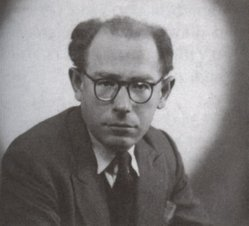
\includegraphics[width=0.6\linewidth]{Robinson}
			\caption{Abraham Robinson}
		\end{subfigure}
		\begin{subfigure}{0.4\textwidth}
			\centering
			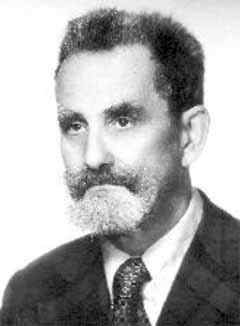
\includegraphics[width=0.4\linewidth]{Los}
			\caption{Jerzy \L o\'s}
		\end{subfigure}
	\end{figure}
\end{frame}

\begin{frame}{Hyperreals} 
We construct a set of \textit{hyperreals}, call it $\hreals$, such that we know three things: \vspace{4pt}
\begin{enumerate} \itemsep = 6pt
	\item $\reals \subseteq \hreals$
	\item $\hreals$ contains at least one infinitesimal $\delta$, such that $0 < \delta$ but $\delta < r$ for any positive real number $r$
	\item Any sentence of first-order logic is true in $\reals$ iff it is true* in $\hreals$
\end{enumerate}
\end{frame}

\begin{frame}{First-Order Logic}
\begin{itemize} \itemsep = 6pt
	\item Our logical language has the following logical symbols:
	\begin{itemize}
		\item $\&$ for ``and''
		\item $\lor$ for ``or''
		\item $\to$ for ``if\ldots then\ldots''
		\item $\leftrightarrow$ for ``if and only if''
		\item $\forall$ for ``for all''
		\item $\exists$ for ``there exists''
		\item $\in$ for set membership
	\end{itemize} 
	\item $5 + 3 = 8 \;\&\; 2^3 = 8$
	\item $1 + 1 = 1 \text{ or } 5 + 7 = 12$
	\item $(\forall x \in \reals)(\exists y \in \nats)(x < y)$
	\item $(\forall x \in \reals)(\forall n \in \nats)(x < \frac{1}{n} \to n < \frac{1}{x})$
\end{itemize}
\end{frame}

\begin{frame}{Transfer Principle}

\end{frame}



\begin{frame}{Infinitesimals}
\begin{itemize}
	\item We construct a set of \textit{hyperreals} $\hreals \supseteq \reals$.
	\item $\hreals$ is ``like'' $\reals$, but it includes \textit{infinitesimals}, elements $\delta$ such that $\delta \neq 0$ but $|\delta| < r$ for every $r \in \reals^+$.
	\item We can add these infinitesimals to other numbers to get things like $1 + \delta$, a number that is ``infinitely close to'' $1$ but not $1$. 
	\item If $|x - y|$ is infinitesimal or $0$, we say $x \simeq y$
	\item If $x \in \hreals$, we denote by $\st(x)$ the \textit{standard part of} $x$, the unique real number that is infinitely close to $x$. $\st(1 + \delta) = 1$. 
	\item We can also take the recipricals of these infinitesimals to get \textit{unbounded} hyperreals, like $\frac{1}{\delta}$. These have no standard part.
	\item We can of course combine all these elements however we'd like. If $\delta$ and $\gamma$ are infinitesimals, we have $\frac{1}{\delta} + 4 + \pi + \gamma \in \hreals$.
\end{itemize}
\end{frame}

\begin{frame}{Derivatives, the way Leibniz intended}
\begin{itemize}
	\item Say $f: \reals \to \reals$. We``extend'' $f$ to $\hr{f}: \hreals \to \hreals$.
	\item Fix $b \in \reals$. Let $\Delta x$ be infinitesimal, and let $\Delta f$ be $\hr{f}(b + \Delta x) - \hr{f}(b)$.
	\item Then define $f'(b) = \stp{\frac{\Delta f}{\Delta x}}$. So $f'(b) \simeq \frac{\Delta f}{\Delta x}$.
	\item \textbf{Example:} Say $f(x) = x^2$. Then we have 
	\begin{align*}
	f'(3) &\simeq \frac{(3 + \Delta x)^2 - 3^2}{\Delta x} = \frac{9 + 6 \Delta x + (\Delta x)^2 - 9}{\Delta x} \\
		&= \frac{6 \Delta x + (\Delta x)^2}{\Delta x} = 6 + \Delta x \simeq 6
	\end{align*}
	\item So $f'(3) \simeq 6$. But these are both real numbers, so their difference can't be infinitesimal. Hence $f'(3) = 6$.
\end{itemize}
\end{frame}

\begin{frame}{Proof: Chain Rule}
Let $f,g: \reals \to \reals$ be differentiable. Let $\Delta x$ be any infinitesimal, and $\Delta g = g(x + \Delta x) - g(x)$. Since $g'(x) = \st(\Delta g / \Delta x)$ is defined, $\Delta g$ must be infinitesimal. Then
\begin{align*}
(f \circ g)'(x) &\simeq \frac{f(g(x + \Delta x)) - f(g(x))}{\Delta x}  \\
	&= \frac{f(g(x) + \Delta g) - f(g(x))}{\Delta g} \cdot \frac{\Delta g}{\Delta x} \\ 
	&\simeq f'(g(x))\cdot g'(x)
\end{align*}
So $(f \circ g)'(x) \simeq f'(g(x)) \cdot g'(x)$. But since both of these numbers are real, they must be identical. \newline

In the case where $\Delta g = 0$, we clearly have $f(g(x) + \Delta g) - f(g(x)) = 0$ and so $(f \circ g)'(x) = 0$.
\end{frame}
\end{document}